\documentclass[12pt]{report}
\usepackage{etoolbox}\AtBeginEnvironment{keyword}{\textbf{Keywords:}\ }\usepackage{float} \usepackage{algorithm2e}\usepackage{algorithm}
\usepackage{listings}
\usepackage{color}
\usepackage{tcolorbox}
\usepackage{mathtools} % mathtools loads the amsmath package automatically
\definecolor{keywords}{rgb}{0.9, 0.0, 0.0}
\definecolor{comments}{rgb}{0.0, 0.5, 0.0}
\definecolor{strings}{rgb}{0.8, 0.2, 0.6}
\definecolor{framecolor}{rgb}{0.4, 0.6, 0.8}  % Light Blue
\definecolor{bgcolor}{rgb}{0.95, 0.95, 0.98}   % Very light cream

\makeatletter
\renewcommand{\@makechapterhead}[1]{%
  {\parindent \z@ \raggedright \normalfont
   \ifnum \c@secnumdepth >\m@ne
     \Huge \bfseries \thechapter\space % Add chapter number and space
   \fi
   #1\par\nobreak
   \vskip 40\p@
  }}
\makeatother

% Define VHDL style
\lstdefinestyle{vhdl}{
    language=VHDL,
    basicstyle=\ttfamily\small,
    keywordstyle=\color{keywords}\bfseries,
    stringstyle=\color{strings},
    commentstyle=\color{comments}\itshape,
    showstringspaces=false,
    breaklines=true,
    numbers=left,
    numberstyle=\tiny\color{gray},
    stepnumber=1,
    numbersep=10pt,
    backgroundcolor=\color{bgcolor},
    xleftmargin=5pt,
    frame=none,
    frameround=fttt,
    captionpos=b,
}

% Language setting
% Replace `english' with e.g. `spanish' to change the document language
\usepackage[english]{babel}
\usepackage{authblk}

% Set page size and margins
% Replace `letterpaper' with `a4paper' for UK/EU standard size
\usepackage[letterpaper,top=2cm,bottom=2cm,left=3cm,right=3cm,marginparwidth=1.75cm]{geometry}

% Useful packages
\usepackage{amsmath}
\usepackage{graphicx}
\usepackage[
    colorlinks=true,  % Color the links
    linkcolor=red,   % Color of internal links
    citecolor=blue,   % Color of citation links
    filecolor=blue,   % Color of file links
    urlcolor=blue     % Color of URL links
]{hyperref}
 % To handle URLs in the bibliography

\title{OpenGL Adventures in Our Solar System}
\author{Marcu-Cristian Petric}
\affil{Technical University of Cluj-Napoca}

\date{\today}



\begin{document}
\maketitle

\begin{abstract}
This project implements a 3D solar system simulation using OpenGL\cite{opengl_programming}, featuring realistic planetary orbits, interactive camera controls, and various visual effects. The system includes all eight planets of our solar system, complete with accurate relative scaling and orbital mechanics. Additional features include a dynamic weather system with rain particles affected by wind, a launchable rocket with physics-based trajectory, and multiple lighting sources. The implementation demonstrates advanced graphics programming concepts including shader management, particle systems, and celestial body movement calculations.
\end{abstract}
\textbf{Keywords:} OpenGL, Computer Graphics, Solar System Simulation, Particle Systems, 3D Graphics Programming


\begingroup
\hypersetup{
    linkcolor = black,
    pdfborder={1 1 1},     % Add borders around links in the ToC
}
\tableofcontents
\endgroup

\chapter{Subject specification}

The project requirements encompass the development of a comprehensive 3D solar system visualization with the following key specifications:

\section{Core Requirements}
\begin{itemize}
    \item Implementation of a complete solar system with eight planets orbiting around a central sun
    \item Realistic orbital mechanics with proper scaling and rotation patterns
    \item Dynamic lighting system featuring:
        \begin{itemize}
            \item Directional light representing sunlight
            \item Multiple point lights around the platform area
            \item Day/night cycle toggle functionality
        \end{itemize}
    \item Interactive camera system allowing free navigation through the scene
    \item Particle system implementation for weather effects
\end{itemize}

\section{Technical Requirements}
\begin{itemize}
    \item Development using OpenGL and C++
    \item Implementation of custom shader programs for lighting and effects
    \item Efficient handling of 3D models and textures
    \item Physics-based animations for rocket launches and particle systems
    \item Shadow mapping for enhanced visual realism
\end{itemize}

\section{User Interaction Requirements}
\begin{itemize}
    \item Camera controls for scene navigation
    \item Keyboard shortcuts for planet tracking
    \item Weather control system
    \item Rocket launch functionality
    \item View mode toggles (wireframe, solid, point)
\end{itemize}

\chapter{Scenario}

\section{Scene and Objects Description}
The solar system simulation recreates our cosmic neighborhood with a focus on both astronomical accuracy and interactive features. At the heart of the scene lies the Sun, serving as both the central celestial body and the primary light source. Eight planets, from Mercury to Neptune, orbit around this central star, each modeled with attention to relative scale and orbital characteristics. Earth is accompanied by its faithful satellite, the Moon, which maintains a realistic orbital pattern around its host planet.

On the terrestrial side, the simulation features a sophisticated launch platform positioned strategically within the scene. This platform serves as the base for rocket operations and is illuminated by an array of point lights implemented as lanterns. These local light sources create an engaging contrast with the Sun's global illumination, especially noticeable during the night cycle. The environment is further enhanced by a dynamic weather system, capable of generating realistic rain patterns that respond to user-controlled wind conditions.

The scene seamlessly integrates interactive elements, with a launchable rocket being the centerpiece of user engagement. This rocket follows physics-based trajectories upon launch, adding a layer of realism to the simulation. The entire environment can be explored through a sophisticated camera system that allows for unrestricted movement throughout the solar system.

\section{Functionalities}
The simulation offers comprehensive user interaction through intuitive control schemes. Navigation through the solar system is achieved through traditional WASD keyboard controls for movement, while mouse input controls the viewing direction. Users can quickly focus on specific planets using number keys 1 through 8, with the camera system automatically tracking the selected celestial body. A zoom function, controlled via the mouse scroll wheel, allows for detailed observation of distant objects.

Environmental control is a key feature of the simulation. Users can toggle rain effects with the R key, while the arrow keys provide precise control over wind direction and strength, affecting the behavior of rain particles. The N key switches between day and night cycles, dramatically altering the lighting conditions and visual atmosphere of the scene.

Visual representation can be modified to suit different observation needs. The F key toggles wireframe mode for structural analysis, while the P key activates point cloud visualization. Rocket launches are initiated with the space bar, sending the vehicle on a physics-governed trajectory through the solar system. These various visualization modes and interactive elements combine to create an engaging and educational space exploration experience.


\chapter{Implementation details}

\section{Functions and Special Algorithms}

\subsection{Orbital Mechanics}
\subsubsection{Possible Solutions}
Two main approaches were considered for implementing planetary orbits:
\begin{itemize}
    \item Full Newtonian gravitational simulation
    \item Simplified parametric circular orbits\cite{kepler_orbits}
\end{itemize}

\subsubsection{The Motivation of the Chosen Approach}
The parametric circular orbit approach was chosen for its computational efficiency and visual clarity, sacrificing physical accuracy for better performance and user experience.

The implementation uses the following equations:
\begin{equation}
\begin{aligned}
x &= x_c + r \cos(\omega t) \\
z &= z_c + r \sin(\omega t) \\
\theta &= \omega t + \theta_0
\end{aligned}
\end{equation}

\subsection{Sun Animation}
\subsubsection{Possible Solutions}
Several approaches were considered for the sun's visual effects:
\begin{itemize}
    \item Particle system-based animation
    \item Texture-based animation
    \item Shader-based procedural animation\cite{graphics_shaders}
\end{itemize}

\subsubsection{The Motivation of the Chosen Approach}
The shader-based procedural animation was selected for its performance and ability to create dynamic, realistic effects without additional texture memory.

The vertex displacement and surface rendering are calculated using:
\begin{equation}
\begin{aligned}
displacement &= A \sin(\omega t + d) \times noise(p) \\
pulse &= \sin(0.5t + 1.5d) \\
flicker &= \sin(2t + 5n) \\
brightness &= 1.0 - 2.0\|texCoord - 0.5\|
\end{aligned}
\end{equation}

\section{Graphics Model}
The graphics pipeline in this project utilizes several key components:

\begin{itemize}
    \item \textbf{Shaders}: Multiple shader programs handle different rendering aspects:
        \begin{itemize}
            \item Main shader for celestial bodies with lighting and shadows
            \item Custom sun shader for solar surface effects
            \item Shadow mapping shader for depth calculations
            \item Rain particle shader for weather effects
        \end{itemize}
    \item \textbf{Textures}: Managed through the Model3D class, including:
        \begin{itemize}
            \item Diffuse textures for surface colors
            \item Specular maps for lighting calculations
            \item Shadow maps for dynamic shadow rendering
        \end{itemize}
    \item \textbf{Framebuffer Objects}: Used for shadow mapping and post-processing effects
\end{itemize}

\section{Data Structures}
The project employs several core data structures:

\begin{itemize}
    \item \textbf{Vertex Structure}:
    \begin{verbatim}
    struct Vertex {
        glm::vec3 Position;
        glm::vec3 Normal;
        glm::vec2 TexCoords;
    };
    \end{verbatim}

    \item \textbf{Mesh Buffers}:
    \begin{verbatim}
    struct Buffers {
        GLuint VAO;
        GLuint VBO;
        GLuint EBO;
    };
    \end{verbatim}

    \item \textbf{Texture Data}:
    \begin{verbatim}
    struct Texture {
        GLuint id;
        string type;
    };
    \end{verbatim}
\end{itemize}

These structures form the foundation for 3D model representation and rendering in the OpenGL pipeline, with careful consideration for memory management and rendering efficiency.

\section{Class hierarchy}
The project's class structure is organized around a core celestial body system with specialized classes for different space objects and supporting functionality:

\begin{itemize}
    \item \textbf{CelestialBody}: The base class for all celestial objects, handling basic orbital mechanics and rendering
        \begin{itemize}
            \item \textbf{Moon}: Extends CelestialBody with specialized orbit behavior around planets
            \item \textbf{Rocket}: Extends CelestialBody with physics-based launch and trajectory calculations
        \end{itemize}
    \item \textbf{Model3D}: Handles 3D model loading and rendering, used by CelestialBody
    \item \textbf{Camera}: Manages view transformations and user perspective control
\end{itemize}

\begin{figure}[H]
\centering
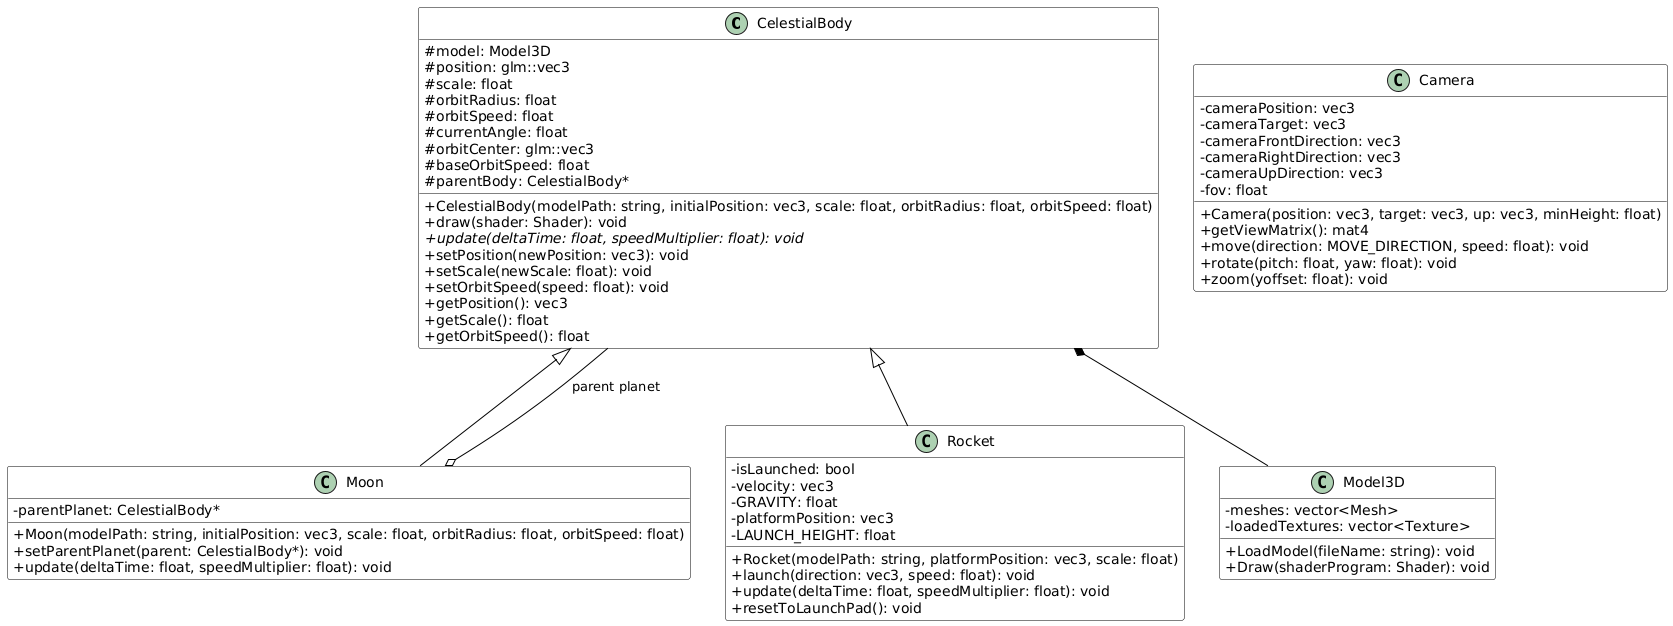
\includegraphics[width=0.8\textwidth]{class_diagram.png}
\caption{UML Class Diagram of the Solar System Simulation}
\label{fig:class_diagram}
\end{figure}

The class hierarchy emphasizes inheritance and composition relationships:
\begin{itemize}
    \item CelestialBody contains a Model3D instance for rendering
    \item Moon and Rocket inherit from CelestialBody, extending its functionality
    \item Moon maintains a reference to its parent planet (CelestialBody)
    \item Camera operates independently but interacts with all rendered objects
\end{itemize}

This structure allows for efficient object management while maintaining clear separation of concerns between rendering, physics, and control systems.

\chapter{User Manual}

\section{Getting Started}
The solar system simulation provides an interactive environment for exploring space. Upon launching the application, you'll be presented with a view of the solar system during daytime.

\begin{figure}[H]
\centering
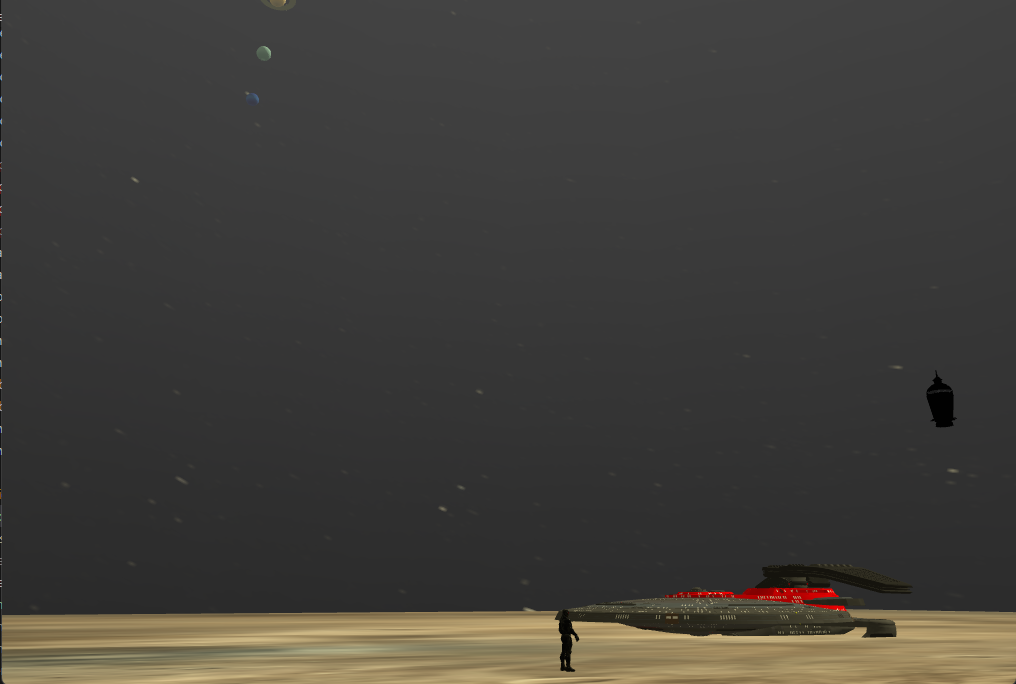
\includegraphics[width=0.8\textwidth]{day.png}
\caption{Solar System - Day View}
\label{fig:day_view}
\end{figure}

\section{Navigation Controls}
\begin{itemize}
    \item \textbf{Basic Movement}:
        \begin{itemize}
            \item W/A/S/D - Move camera forward/left/backward/right
            \item Mouse Movement - Look around
            \item Mouse Scroll - Zoom in/out
        \end{itemize}
    \item \textbf{Planet Selection}:
        \begin{itemize}
            \item Keys 1-8 - Focus on specific planets (Mercury through Neptune)
        \end{itemize}
\end{itemize}

\begin{figure}[H]
\centering
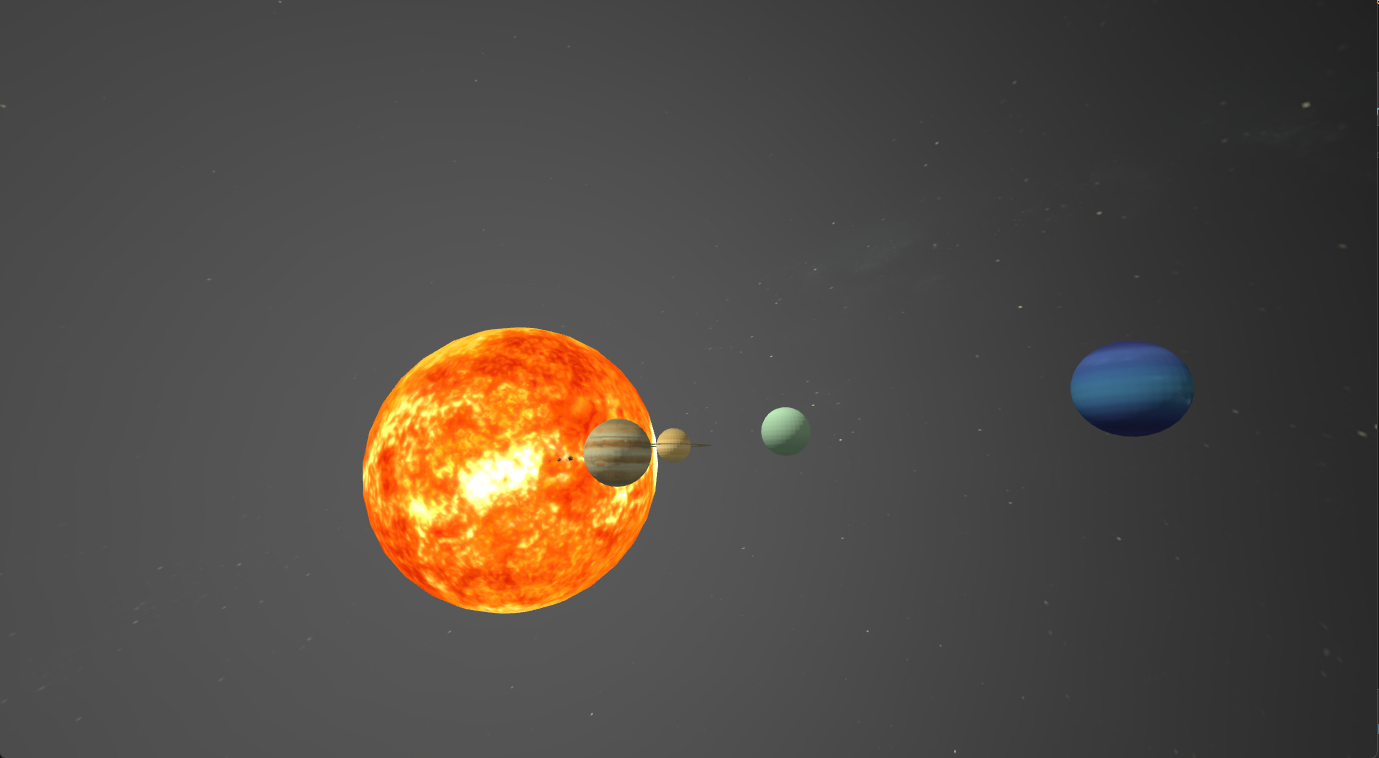
\includegraphics[width=0.8\textwidth]{planets.png}
\caption{Planetary View}
\label{fig:planets_view}
\end{figure}

\section{Special Features}
\begin{itemize}
    \item \textbf{Environment Controls}:
        \begin{itemize}
            \item N - Toggle between day and night modes
            \item R - Toggle rain effect
            \item Arrow Keys - Control wind direction
        \end{itemize}
    \item \textbf{Display Modes}:
        \begin{itemize}
            \item F - Toggle wireframe mode
            \item P - Toggle point cloud mode
        \end{itemize}
    \item \textbf{Interactive Elements}:
        \begin{itemize}
            \item Space Bar - Launch rocket
        \end{itemize}
\end{itemize}

\begin{figure}[H]
\centering
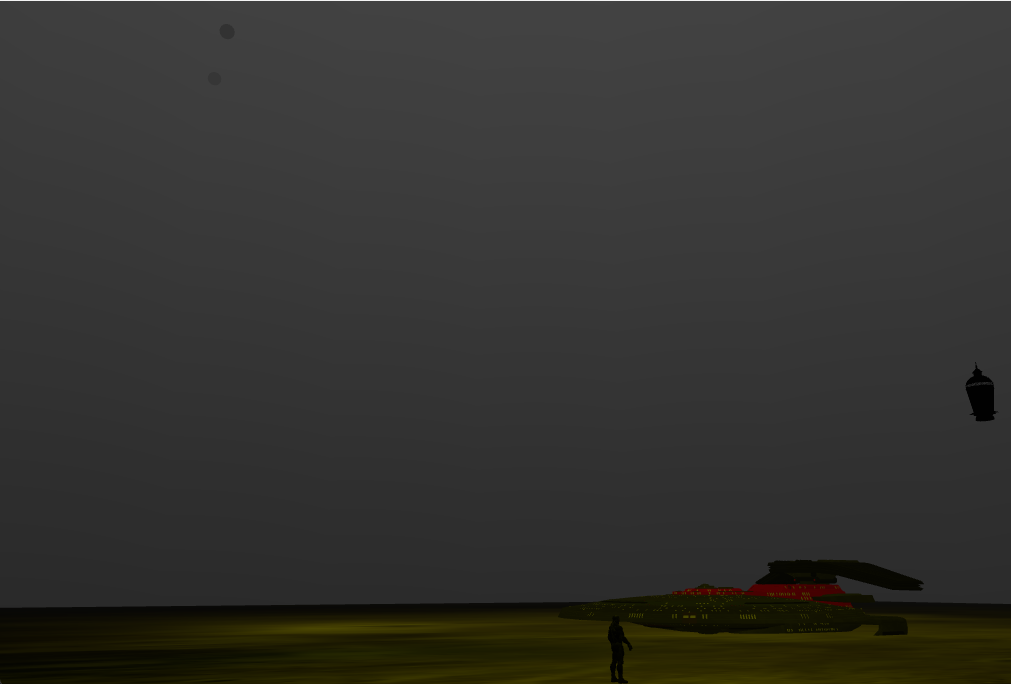
\includegraphics[width=0.8\textwidth]{night.png}
\caption{Solar System - Night View}
\label{fig:night_view}
\end{figure}

\section{Tips and Tricks}
\begin{itemize}
    \item Hold Shift while moving to increase movement speed
    \item Use the mouse scroll wheel to adjust your view distance
    \item The rocket will automatically reset when it hits the ground
    \item Rain particles are affected by wind direction - experiment with different combinations
\end{itemize}

\chapter{Conclusions and Further Developments}

The Solar System simulation project successfully demonstrates the implementation of a complex 3D graphics application using OpenGL. The project achieves its primary objectives of creating an interactive, educational tool for exploring planetary motion and space physics.

Key achievements include:
\begin{itemize}
    \item Implementation of realistic orbital mechanics for planets and moons
    \item Development of a dynamic sun shader with realistic surface effects
    \item Creation of an interactive camera system with smooth tracking capabilities
    \item Integration of environmental effects including day/night cycles and weather
    \item Physics-based rocket launch system with trajectory calculations
\end{itemize}

Potential areas for future development include:
\begin{itemize}
    \item \textbf{Enhanced Physics Simulation}:
        \begin{itemize}
            \item Implementation of gravitational interactions between bodies
            \item More accurate orbital mechanics using Kepler's laws
            \item Collision detection and response for the rocket
        \end{itemize}
    \item \textbf{Visual Improvements}:
        \begin{itemize}
            \item Advanced atmospheric effects for planets
            \item Asteroid belt visualization
            \item More detailed planet surface textures
        \end{itemize}
    \item \textbf{Interactive Features}:
        \begin{itemize}
            \item Multiple camera viewpoints
            \item Educational information display for celestial bodies
            \item Mission-based gameplay elements
        \end{itemize}
\end{itemize}

The modular architecture of the project allows for these future enhancements while maintaining performance and code maintainability. The current implementation provides a solid foundation for expanding the simulation's capabilities and educational value.


\bibliographystyle{alphaurl}  % Citation style
\bibliography{sample}  % Your .bib file

\end{document}